\section{去雾算法理论方法}
\label{s2}

\subsection{雾与霾的成因及影响}
雾,是一种常见的气象,被称为在地面上的云。当潮湿的空气中遇到灰尘等凝结核时,水蒸气会凝结,在冷凝过程中,水蒸气分子结合形成悬浮在空气中的小水滴与小冰晶,雾需要一定的湿度才会形成。雾可能会突然形成,然后很快消失。霾,是指原因不明的因大量烟、尘等微粒悬浮而形成的浑浊现象。霾的核心物质是空气中悬浮的灰尘颗粒,气象学上称为气溶胶颗粒,与雾不同的是,霾在干燥的时候更容易出现。

当烟、尘等微粒累积超过大气的调节能力时,雾霾就会在微风与大气稳定的情况下出现。由于存在大气吸收和散射,霾、雾和烟雾的现象,入射光与大气光混合,环境光被大气粒子反射到视线中。图像出现退化的问题,失去对比度和色彩保真度。雾与霾不但影响人的身心健康,还会影响基于视觉系统的各类服务,影响生活生产的各方各面,在生产、安全等方面存在巨大隐患。因此,图像去雾算法拥有巨大的需求。

\subsection{大气散射物理模型}
\label{subsec-atsm}
\begin{figure}[htbp]
    \centering
    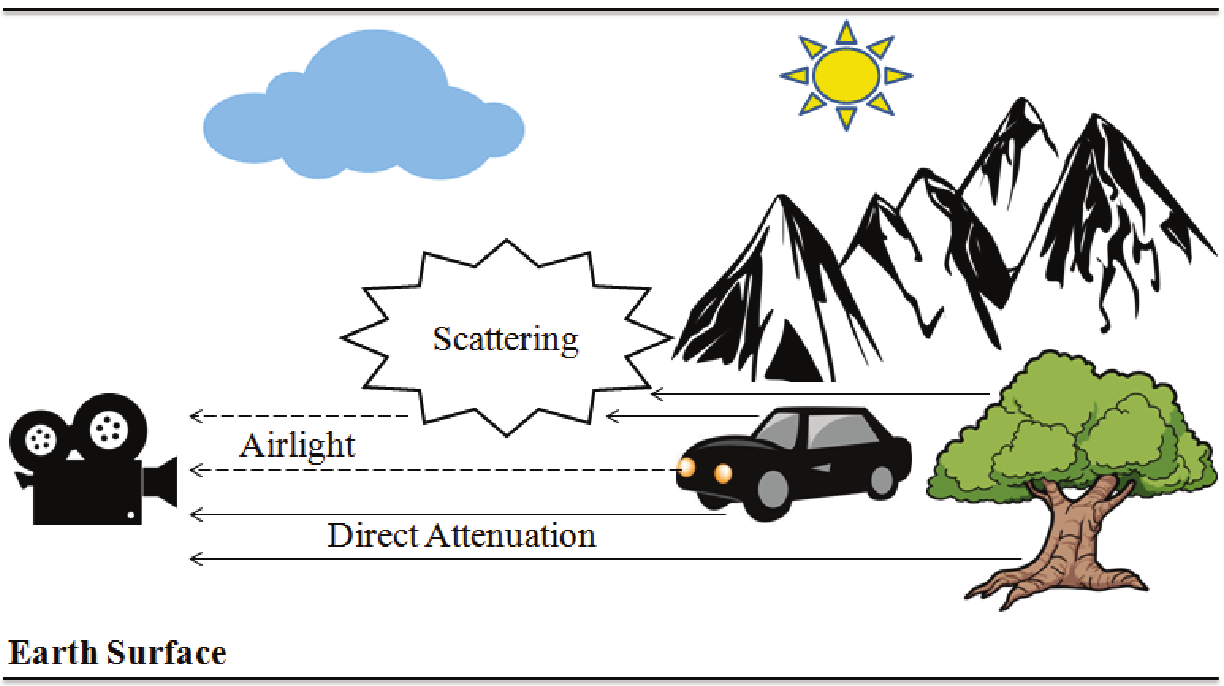
\includegraphics[width=0.8\textwidth]{./imgs/g167.png}
    \caption{大气散射物理模型}
    \label{fig-astm}
 \end{figure}

解决SID的基本模型是ATSM\cite{narasimhan2004models}。 ATSM考虑了散射光对恶劣天气下图像形成的影响。恶劣天气下的成像过程如图\ref{fig-astm}所示。物体表面反射入射的太阳光。一部分反射光到达相机(直接衰减),一部分反射光被大气粒子散射(大气光)。因此,相机接收到的图像是散射光和非散射光的总和。 ATSM模型可转化为数学表示\cite{narasimhan2004models},如公式\eqref{eq-astm}所示。

\begin{equation}
    I_h^c(x,y) = \underbrace{I_n^c(x,y)\times t_r(x,y)}_{\text{传输衰减}} + \underbrace{A_r^c(x,y)\times t_r(x,y)}_{\text{大气光}}
    \label{eq-astm}
\end{equation}

其中,$(x,y)$是图像中像素点的坐标,$c\in\text{(red,green,blue)}$是颜色通道,$I_n$是无雾图像,$I_h$是雾化图像,$A_r$是全局值大气光。位置 $(x,y)$处的透射率(非散射光比例)由 $t_r (x, y)$ 表示。公式\eqref{eq-astm2}描述了光如何在大雾天气中传输。

\begin{equation}
    t_r (x, y) = e^{-\gamma\text{Depth}(x, y)}
    \label{eq-astm2}
\end{equation}

其中,$0\leq\text{Depth}(x, y)\leq\infty$为场景点的景深,$\gamma$是散射系数。公式\eqref{eq-astm2}中可知随着景深的增大传输到相机的光减小。 SID 的主要任务是从单个模糊图像\cite{he.tang201112}估计 $t_r (x, y)$ 和$A_r$。将$t_r (x, y)$和$A_r$的值代入公式\eqref{eq-astm}即可得到无雾图像。无雾图像由于传输$t_r (x, y)$和附加大气光 $A^c_r\times (1 − t_r (x, y))$产生退化。因此,高质量SID非常需要准确的估计传输函数。雾度的浓度的估计由公式\eqref{eq-astm2}中的 $\gamma$ 和 Depth$(x,y)$控制。现有的去雾方法使用公式\eqref{eq-astm}或\eqref{eq-astm2} 来估计 $t_r (x, y)$。然而,由于估计的$A_r$和DCP在某些区域(如天空)的无效性,公式\eqref{eq-astm}引入了重建误差,同时公式\eqref{eq-astm2}的$\gamma$也会造成传输误差,也是一个重要的超参数,$\gamma$设置的合理与否直接影响传输函数的估计效果(默认为1)。

\subsection{去雾效果评价方法}
与其他计算机视觉的领域不一样,图像去雾效果的评价较为特殊,各个算法中的度量指标并不统一,没有一个严格的评价标准,但是大体上都分为两部分:主观评价和客观评价。

\subsubsection{主观评价方法}
主观评价的方法是依赖于观察测试人员的直观感受评价,评价一张图像处理后的质量,需要对多个观察测试人员的评价进行归一化即为该图像的评分。在图像去雾中,主观评价方法可分为两种,一种是对合成有雾图像的去雾评价,像这样有参照的无雾图像的属于绝对评价方法;另一种是对真实情况的有雾图像的去雾评价,像这样没有参照的无雾图像的属于相对评价方法。观察者根据自身对图像的视觉感受、图像质量、颜色与细节的模糊程度来判断去雾效果。虽然主观评价方法原理简单又能直接体现去雾效果,但是碍于观察测试者的自身情况不同,评价的标准也不尽相同,并且操作起来费时费力,导致主观评价并不能精准的反映去雾效果,也很难应用在类似于无人驾驶的实时图像去雾上。

\subsubsection{客观评价方法}
本文的客观评价方法主要基于两个计算机视觉中常用的度量:峰值信噪比(Peak Signal to Noise Ratio,PSNR)与结构相似性(Structural Similarity Index,SSIM)\cite{Zhou2004}。客观评价避免了人为主观的影响,并且对每一副图像都有相同的评价,可以批量处理与综合评价,反映整体去雾水平。在客观评价的实验中,我们采用了RESIDE\cite{li2019benchmarking}\footnote{https://sites.google.com/view/reside-dehaze-datasets/reside-standard}中的SOTS(Synthetic Objective Testing Set)户外数据集,数据集包括原图与加雾图,对去雾算法的评价方式为:结果客观评价方法的大致步骤就是,将处理后的图像作为输入,经客观评价模型计算后,再与无雾图像在数据上进行分析评价,如图\ref{fig6}所示。

\begin{figure}[htbp]
   \centering
   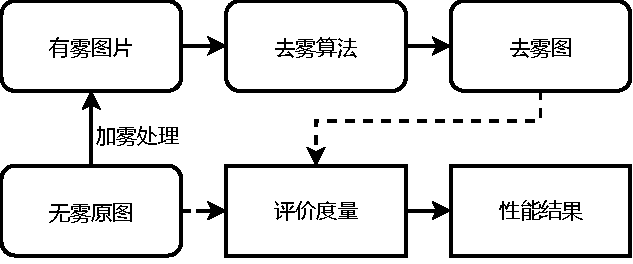
\includegraphics[width=0.8\textwidth]{./imgs/metric.pdf}
   \caption{客观评价方法流程图}
   \label{fig6}
\end{figure}


PSNR是客观评价方法的一种鉴别图像处理结果的画质的客观方法,可以看作评价图像的客观标准。表达式如公式\eqref{eq-psnr}所示:

\begin{equation}
    \text{MSE} = \frac{1}{MN\times\text{channels}}\sum\limits_{\dim}^{\text{channels}}\sum\limits_{i}^{M}\sum\limits_{j}^{N}(I_x^{(i,j,\dim)} -I_y^{(i,j,\dim)})^2,
    \label{eq-mse}
\end{equation}

\begin{equation}
    \text{PSNR} = 10\times\log_{10}\left(\frac{(2^n-1)^2}{\text{MSE}}\right).
    \label{eq-psnr}
\end{equation}

由上式可知,PSNR在作为图像品质的指标的时候,其实是均方误差(mean square error,MSE)\eqref{eq-mse}的一种变体,其中MSE的$n$指的是图像的位数。去雾后的图像与原图越相近,均方误差越小,PSNR 的值越高。图像去雾任务中,输出的图像和原图像会存在很大不同,PSNR 的大小无法和人评
价图像质量的视觉感受完全一致,有时候人眼看去雾效果差的图像,其 PSNR 分
数反而会相对较高。但是在这是因为人对图像某一区域的视觉感知结果会收到区域周围
的对比度、亮度等影响

SSIM是衡量两幅图像相似程度的指标,它的数值代表了两个图像之间的相似性。人类对像素的绝对亮度/颜色不敏感,但对边缘和纹理的位置非常敏感。SSIM通过主要关注边缘和纹理相似性来模仿人类感知。其表达式如公式\eqref{eq-ssim}所示:
\begin{equation}
    \hbox{SSIM}(I_x,I_y) = \frac{(2\mu_x\mu_y + c_1)(2\sigma_{xy} + c_2)}{(\mu_x^2 + \mu_y^2 + c_1)(\sigma_x^2 + \sigma_y^2 + c_2)}.
    \label{eq-ssim}
\end{equation}
其中$\mu_x$和$\mu_x$是图像像素集合$I_x$与$I_y$的平均像素亮度,$\sigma_x^2$与$\sigma_y^2$是$I_x$与$I_y$的方差,$\sigma_{xy}$是$I_x$与$I_y$的协方差;$c_1 = (k_1L)^2$, $c_2 = (k_2L)^2$是两个常数,确保除法中不存在除以0的情况,$L$是像素的取值范围(亮度格式)、默认情况下$ k_1 $$k_2 $的值分别为$0.01$与$0.03$.

在客观评价去雾效果时候,需要结合PSNR和SSIM两个评价指标,共同衡量去雾效果的优劣。